\textcolor{red}{THIS IS UNEDITED AND SHOULD NOT BE READ YET - Placeholder}
	
Coala's API adds only 5 syntactic constructs to C-based languages: \texttt{COALA\_TASK}, used to declare a new task; \texttt{COALA\_PV}, used to declare a new protected variable; \texttt{COALA\_NEXT\_TASK} used to mark the next task to be scheduled after the currently executing one completes; \texttt{RP}, used to mark a protected variable read; \texttt{WP}, used to mark a protected variable write.

Moreover, the programmer is required to explicitly call two API functions inside the main body: \texttt{COALA\_INIT}, passing the global initialization task to run upon the first boot as argument; \texttt{COALA\_RUN}, which hands the control to Coala's scheduler.

Finally, when the programmes intends to typedef a struct, to use it as a protected variable, they need to declare each structure's member by using the following macro: \texttt{COALA\_SM}, used to ensure proper memory alignment required by Coala's page handler.

The following table summarizes Coala's API methods and their arguments. $T$ denotes the set of all tasks, while $V$ denotes the set of all protected variables. These methods trigger specific kernel functions, whose detailed implementation is given in the next paragraph.

\begin{table}
\centering
\begin{tabular}{| c | c |}
	\hline
	\textbf{Method} & \textbf{Arguments} \\
	\hline\hline
	\texttt{COALA\_TASK}($t$, $w_t$) & $t \in T$: new task name, $w_t$: weight of task $t$ \\
	\hline
	\texttt{COALA\_PV}(type, $v$ [, size]) & type: var. type, $v \in V$: new protected var. name, size (optional)  array size\\
	\hline
	\texttt{COALA\_NEXT\_TASK}($t$) & $t \in T$ : next task to schedule\\
	\hline
	$u$ := RP($v$) & $v \in V$: protected variable to be read, $u$: value \\
	\hline	
	WP($v$) := $u$ &  $v \in V$: protected variable to be written, $u$: value \\
	\hline
	\texttt{COALA\_INIT}(t) & $t \in T$: task to be scheduled on first boot \\
	\hline
	\texttt{COALA\_RUN}() & {} \\
	\hline
	\texttt{COALA\_SM}(type, $m$ [, size]) &  type: struct member's type, $m$: struct member's name, size (optional): array size \\
	\hline
\end{tabular}
\caption{Coala API}
\label{table:coala_api}
\end{table}

An example usage of Coala’s API is given in the following code snippet. (TBW)

\subsection{Kernel functions implementation}

New tasks. The API method \texttt{COALA\_TASK} statically allocates a non-volatile constant variable holding the task weight, and declares a void function with the name passed as an argument.

New protected variables. The API method \texttt{COALA\_PV} statically allocates (and aligns in memory) a non-volatile variable, whose address will be used by RP and WP to locate the most recent location of the variable itself, which could be either the location of the variable in volatile memory or its location in non-volatile memory.

Task transitions. By calling \texttt{COALA\_NEXT\_TASK}, the user tells Coala’s scheduler what task to execute next. Note that the currently executing is not interrupted, and only once it completes the next task is run.

Protected reads and writes. When RP and WP are used, Coala searches the volatile memory for the page the protected variable belongs to. If such page is not found in RAM, then a page fault occurs, and the page is fetched from the non-volatile memory. The two functions return a handle to the variable’s volatile memory location. Unlike RP, WP marks the page being written as dirty, so that it can be committed to its non-volatile location.

Initialization and origin task. The behavior of the method \texttt{COALA\_INIT} is very similar to \texttt{COALA\_NEXT\_TASK}, with the addition that all the preliminary kernel initializations are performed inside this function. Moreover, the origin task is scheduled only upon the first boot.

Execution. The application control is passed to Coala’s scheduler by calling \texttt{COALA\_RUN} at the end of the main function. A high-level state machine of the scheduler is depicted in Figure \textcolor{red}{[draw and ref figure]}. Depending on the coalescing algorithm, state transitions follow a different pattern.

\subsection{Paging}

Memory virtualization. Working (volatile) buffer, store and shadow (non-volatile) buffers. No major changes since last version.

Page allocation and page tags. When the application accesses a protected variable with RP or WP, Coala has to search for the variable in RAM first, and in non-volatile memory if it not found in RAM. Actually, the kernel searches for pages, not single variables. A page search can be very fast if each page is identified by a unique tag, and if every variable belonging to a page bears the tag in its address. Thus, retrieving a page tag from a protected variable’s address boils down to extracting the upper bits of the address itself. The remaining lower bits denote the variable’s offset in its page.

\begin{figure}
	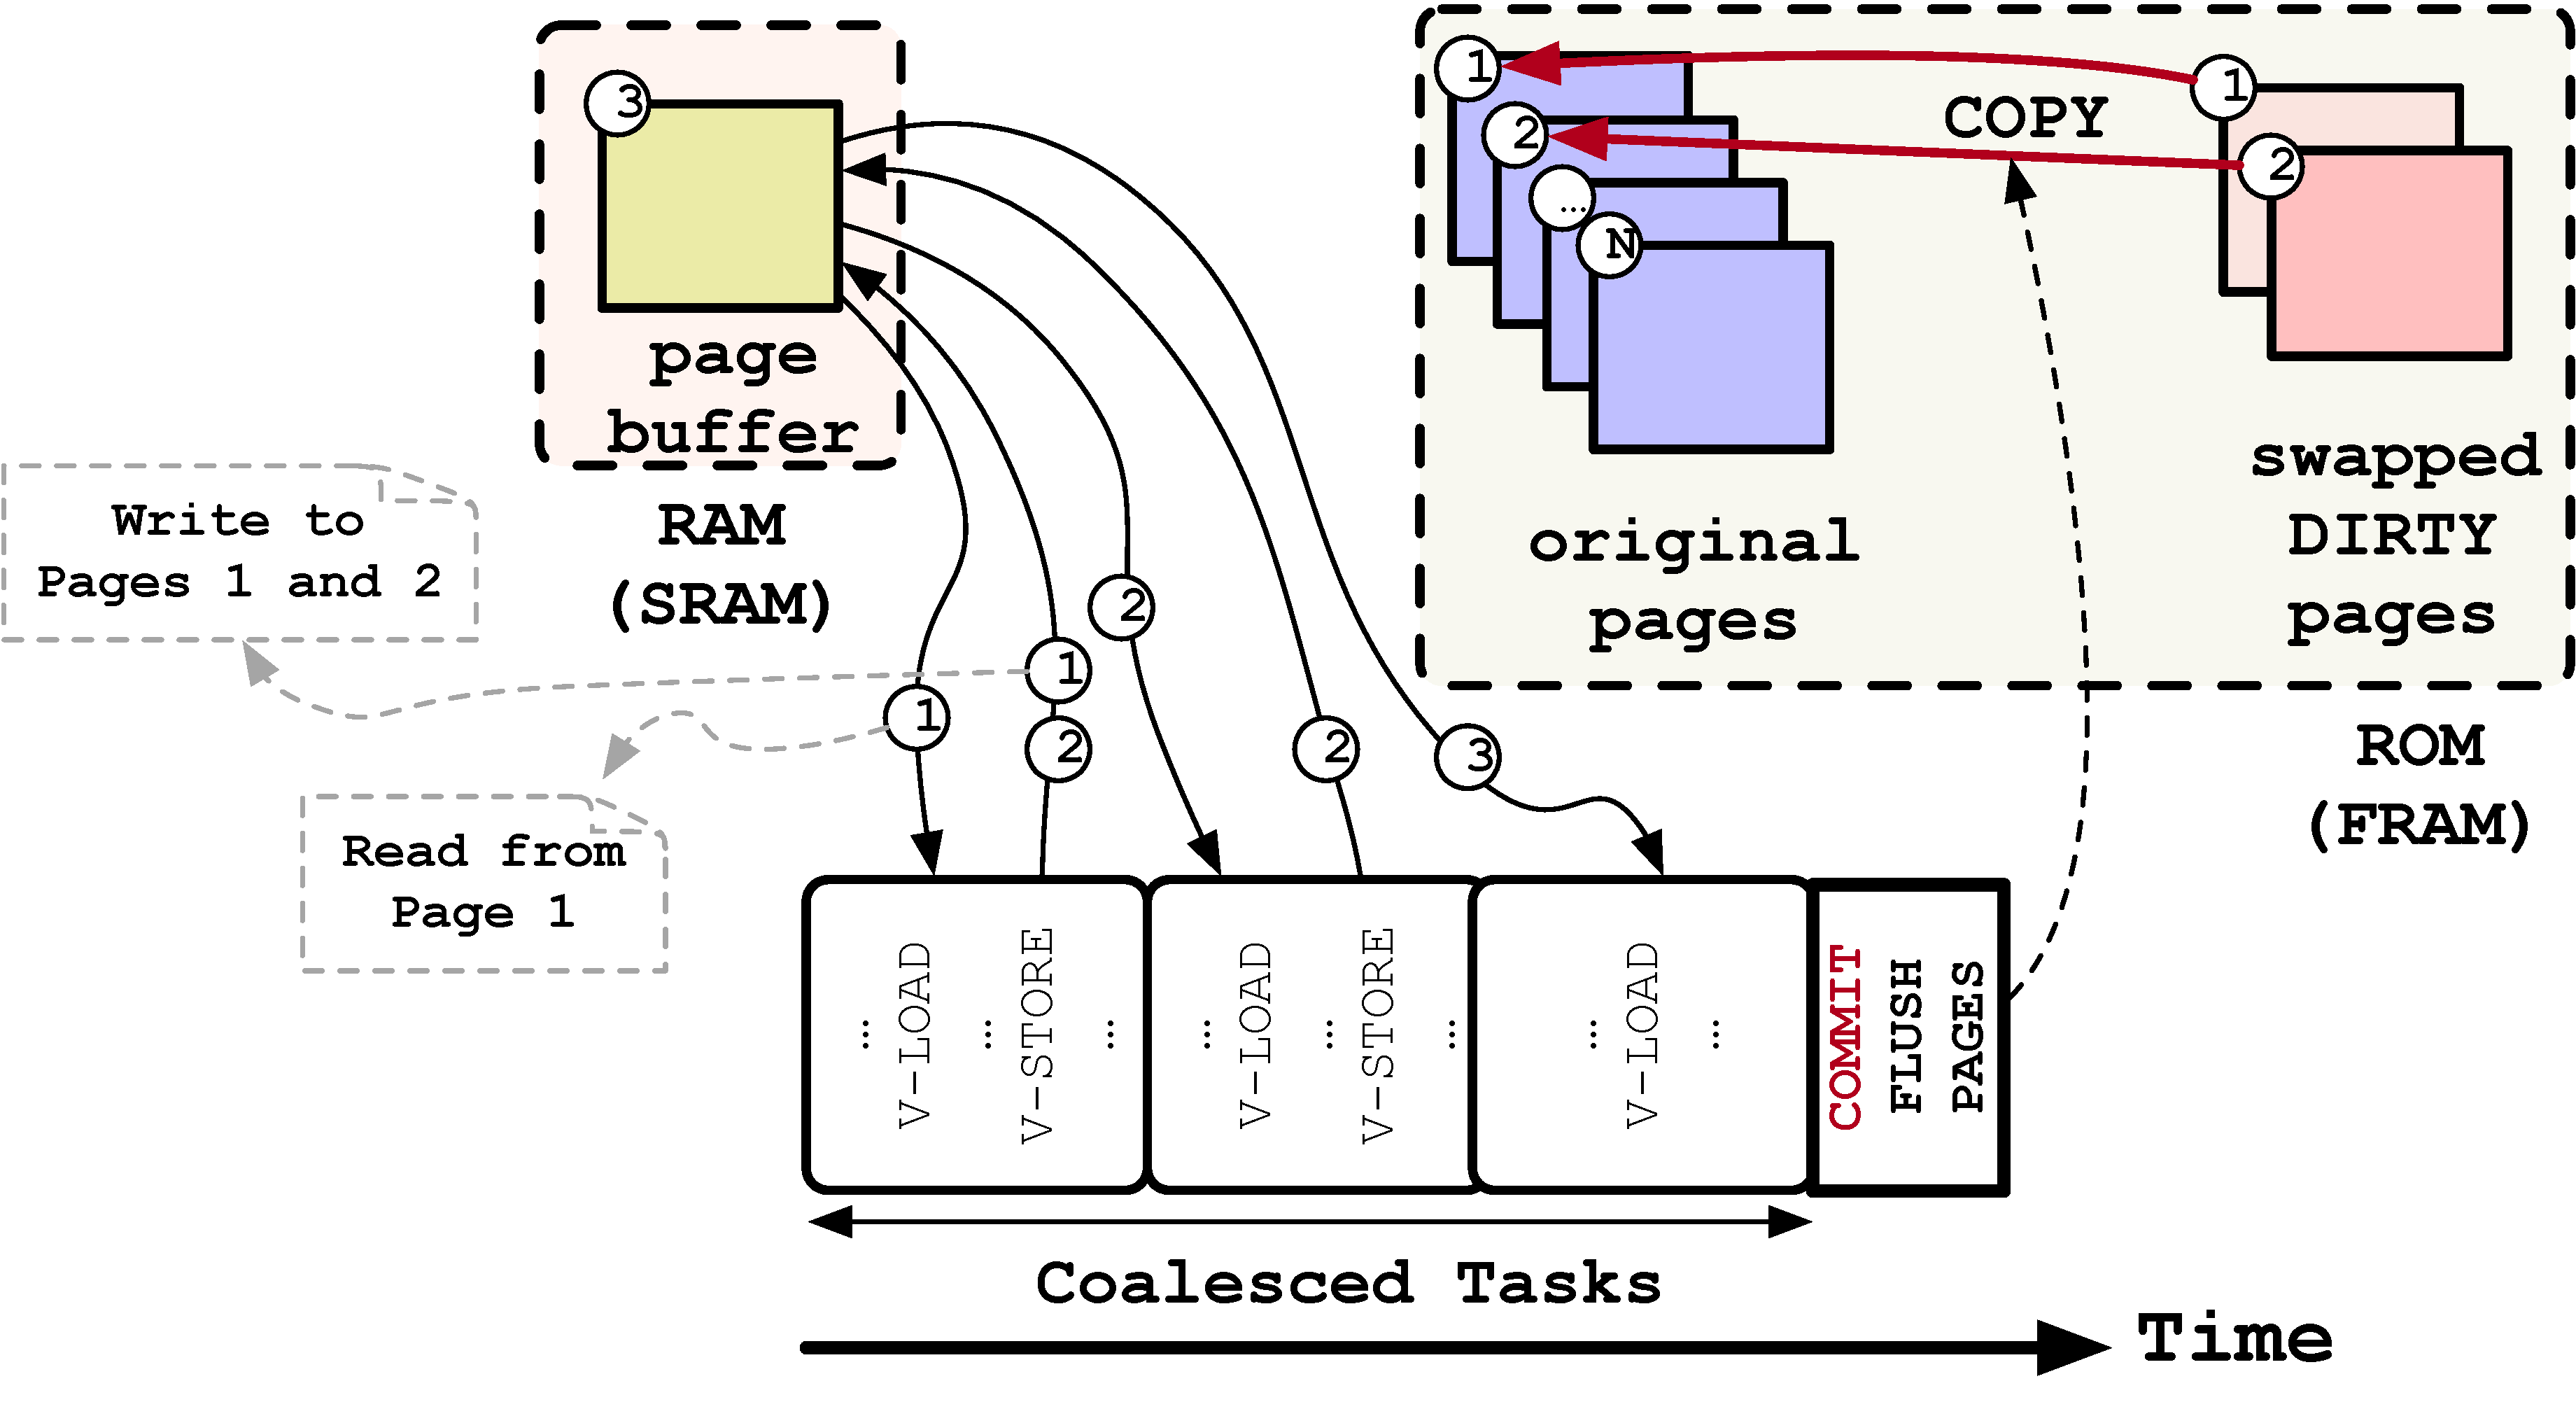
\includegraphics[width=0.9\textwidth]{figures/graffle/paging.pdf}
	\caption{Illustration of page tags \textcolor{red}{to be drawn}}
\end{figure}

In order to obtain unique page tags, some alignment requirements have to be met. First, the page size $S$ has to be a power of two. Moreover, pages in non-volatile memory have to be aligned by $S$. In the example above, $S$ is 256, and every page’s first address is a multiple of 256. Note that, by aligning pages by $2n$, the alignment is also valid for all sizes $2^x$ with $x \leq n$.

Page fault and page swap (with DMA). When a page is not found in RAM, it is fetched from FRAM. No major changes since last version.

\subsection{Scheduling and Committing}

Target budget initialization. Upon a reboot, the target budget (or target coalesced task size) has to be updated depending on the coalescing strategy [...].

Coalescing state recall. The last (coalesced) task has to be recalled. More specifically, the function pointer of the last coalesced task has to be retrieved from NV memory, where is had been saved during the last successful commit. [...].

Partial execution restoration. In case there is a valid partial execution checkpoint, the program has to resume from there [...].

Coalesced scheduling. Static tasks are coalesced and run [...].

Intermediate commit and ultimate commit. When a coalesced task is successfully run to completion, all the dirty pages in SRAM have to be persistently saved to non-volatile memory. Since last version, no major changes were made to the intermediate commit (SRAM to shadow buffer), but an optimization was applied to the ultimate commit (shadow buffer to store buffer). Store buffer and shadow buffer used to be physically separated in memory. Now, the role of a block of memory (i.e. a page) is interchangeable, meaning that, during the ultimate commit, the shadow buffer pages that were written during the previous commit phase become store buffer pages, and their relative store buffer pages become shadow buffer pages. A page’s role is retrieved using an indirection table, i.e. an array that holds a zero for all the pages whose store buffer resides in the lower memory block, and a one for all the pages whose store buffer is located in the upper memory block. This allows for a lighter commit process, since fewer page moves are performed.

\begin{figure}
	\caption{Intermediate commit and ultimate commit Illustration \textcolor{red}{to be drawn}}
\end{figure}

Target budget update. Before starting a new coalesced task, the target budget (or target coalesced task size) has to be updated depending on the coalescing strategy [...].

\textcolor{red}{API of the partial commit needs to be explained as well}